\documentclass[12pt]{article}
\usepackage{tikz}

\author{Binit Pandit}
\title{Drawing in \LaTeX\ using PGF/TikZ}
\date{}

\begin{document}
\maketitle\vskip-25pt\hrule\vskip10pt

%\begin{tikzpicture}[options]
%\path[optional1][optional1] <specifications> ;
%\end{tikzpicture}

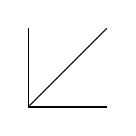
\begin{tikzpicture}
\draw (0,0) -- (1,0) ;
\draw (0,0) -- (0,1) ;
\draw (0,0) -- (1,1) ;
\end{tikzpicture}

\vskip25pt

\begin{tikzpicture}
\draw (1,0) -- (0,0) -- (0,1) ;
\end{tikzpicture}

\vskip25pt

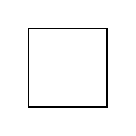
\begin{tikzpicture}
\draw (0,0) -- (1,0) -- (1,1) -- (0,1) -- (0,0);
\end{tikzpicture}

\vskip25pt
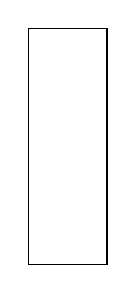
\begin{tikzpicture}
\draw (0,0) rectangle(1,3);
\end{tikzpicture}

\vskip25pt
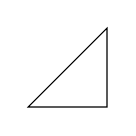
\begin{tikzpicture}
\draw (0,0)--(1,0)--(1,1)--cycle;
\end{tikzpicture}

\vskip25pt
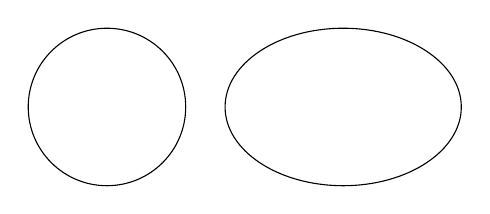
\begin{tikzpicture}
\draw (0,0) circle[radius=1cm];
\draw (3,0) circle[x radius=1.5cm, y radius=1cm];
\end{tikzpicture}

\vskip25pt
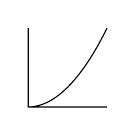
\begin{tikzpicture}
\draw (1,0)--(0,0)--(0,1) (0,0)parabola(1,1);
\end{tikzpicture}

\end{document}
